%
% Bilderserie zur wandernden Rechteckfunktion
%
\begin{figure}
\centering
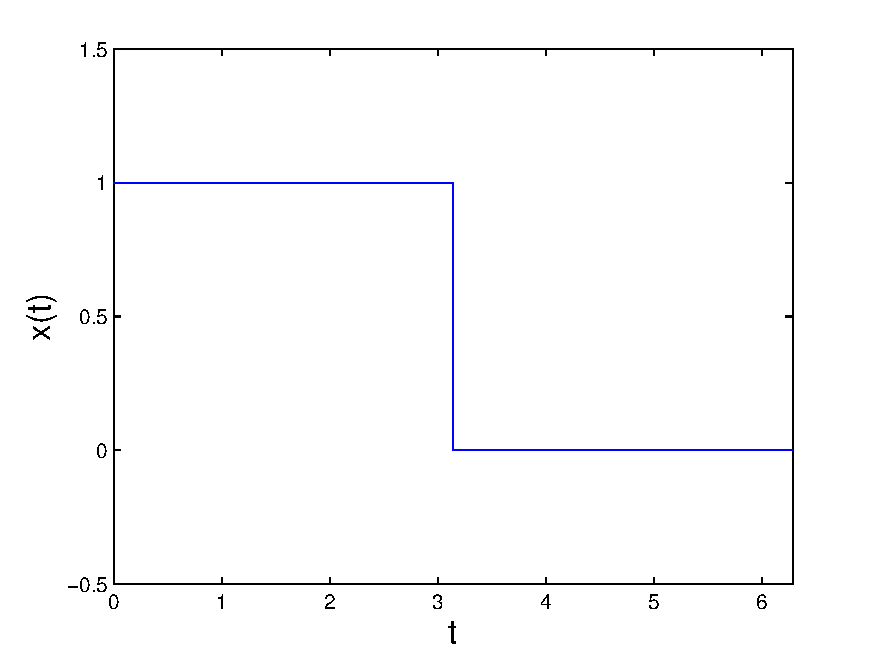
\includegraphics[width=0.45\textwidth]{kugel/kSpektrum/Rechteck1_1.pdf}
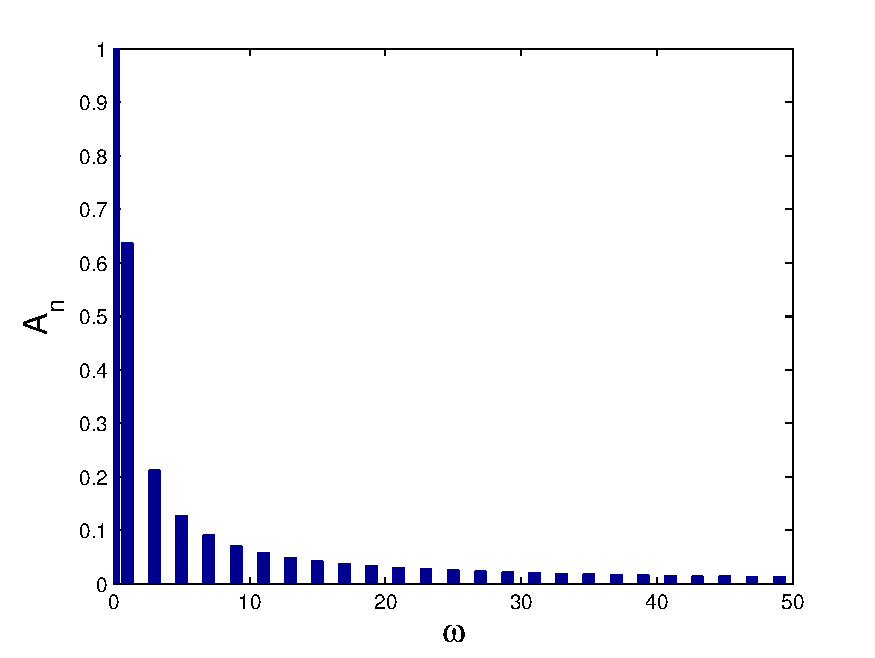
\includegraphics[width=0.45\textwidth]{kugel/kSpektrum/Rechteck1_2.pdf}
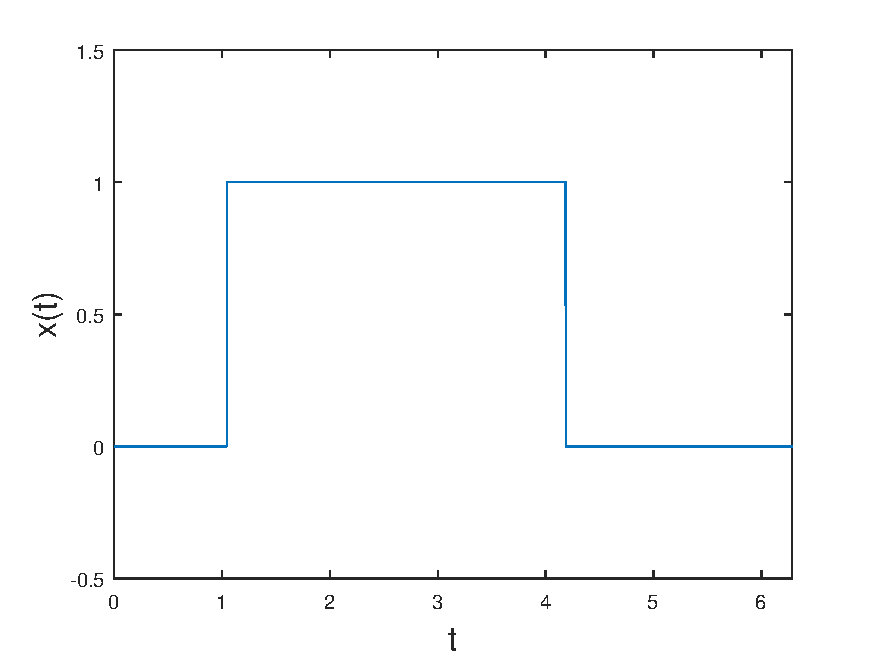
\includegraphics[width=0.45\textwidth]{kugel/kSpektrum/Rechteck2_1.pdf}
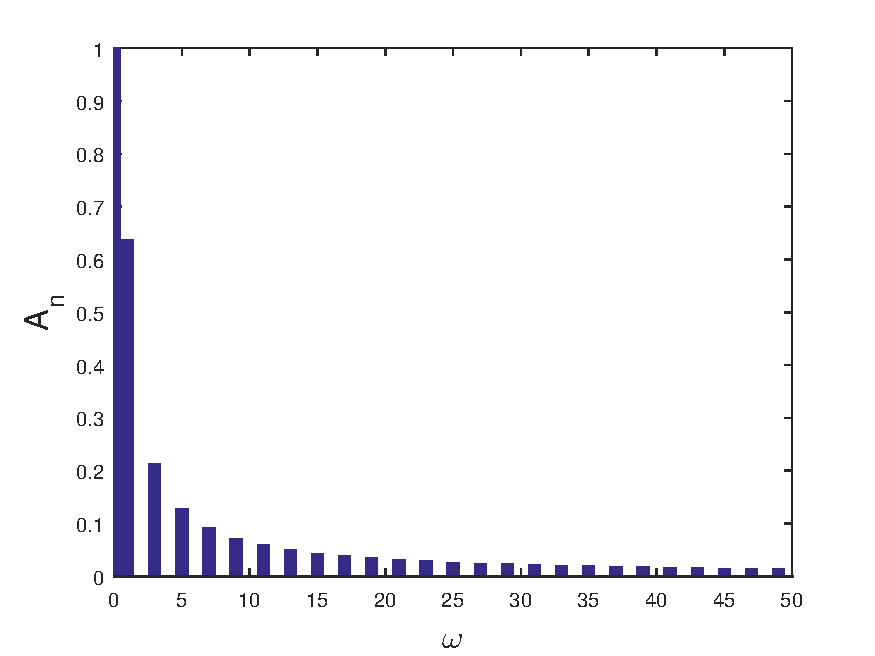
\includegraphics[width=0.45\textwidth]{kugel/kSpektrum/Rechteck2_2.pdf}
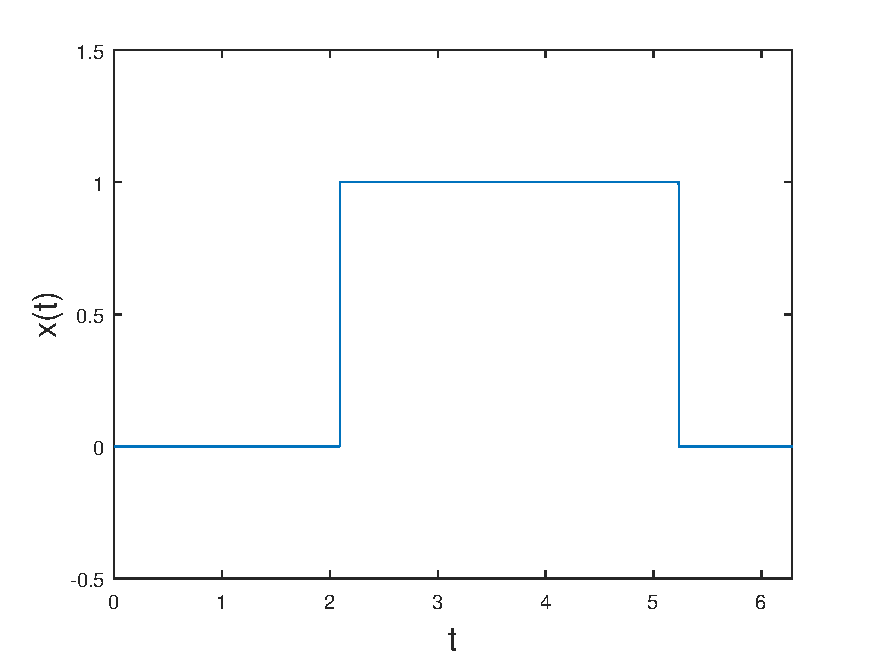
\includegraphics[width=0.45\textwidth]{kugel/kSpektrum/Rechteck3_1.pdf}
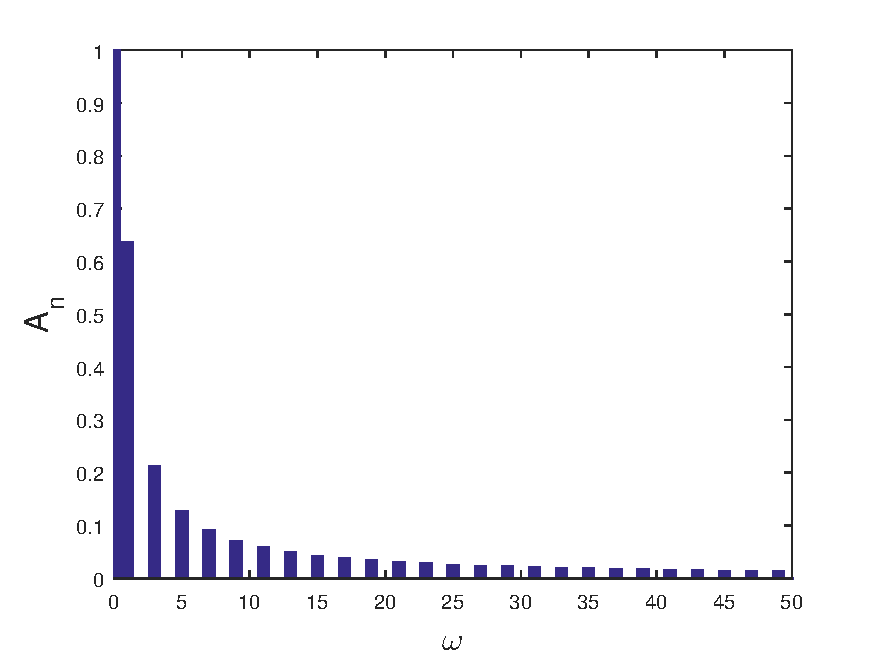
\includegraphics[width=0.45\textwidth]{kugel/kSpektrum/Rechteck3_2.pdf}
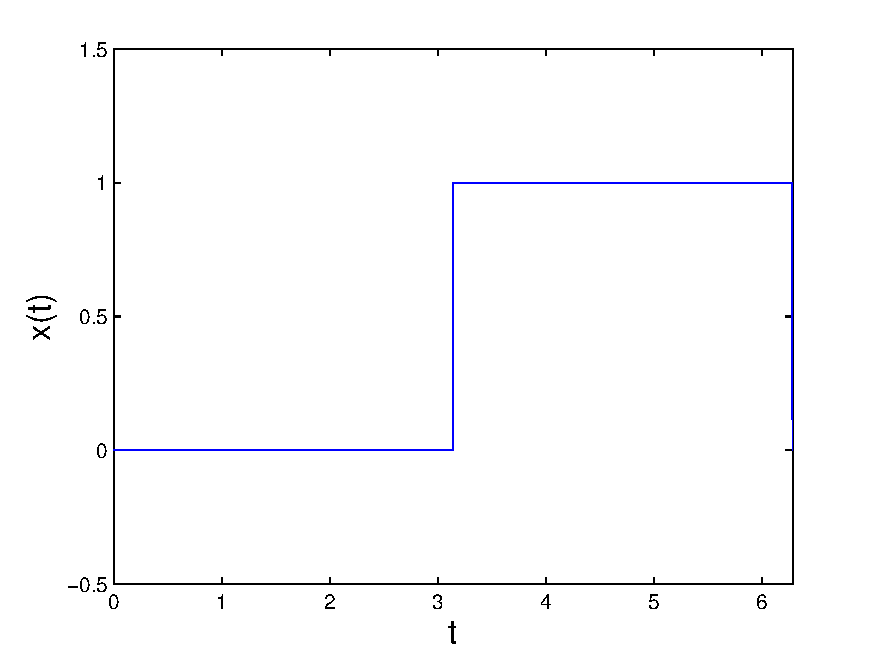
\includegraphics[width=0.45\textwidth]{kugel/kSpektrum/Rechteck4_1.pdf}
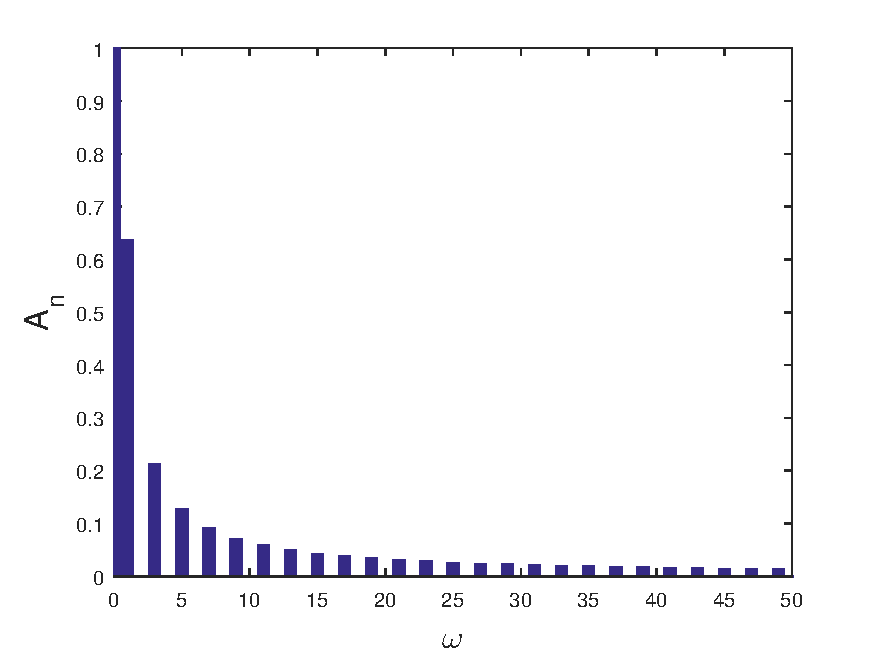
\includegraphics[width=0.45\textwidth]{kugel/kSpektrum/Rechteck4_2.pdf}
\caption{Wandernde Rechteckfunktion
\label{skript:Spektrum1}}
\end{figure}
\begin{figure}
\centering
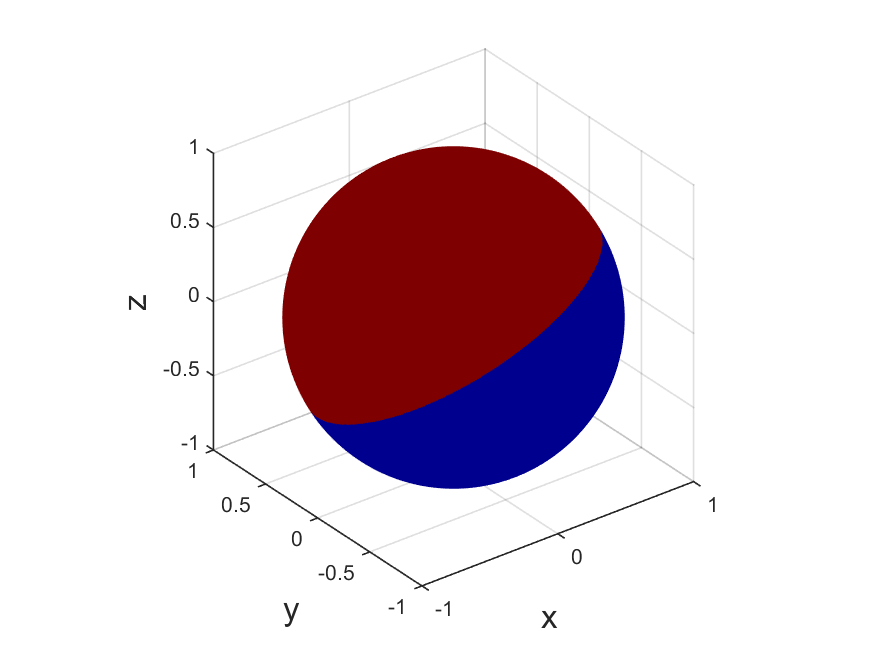
\includegraphics[width=0.45\textwidth]{kugel/kSpektrum/Kugel_1_1.pdf}
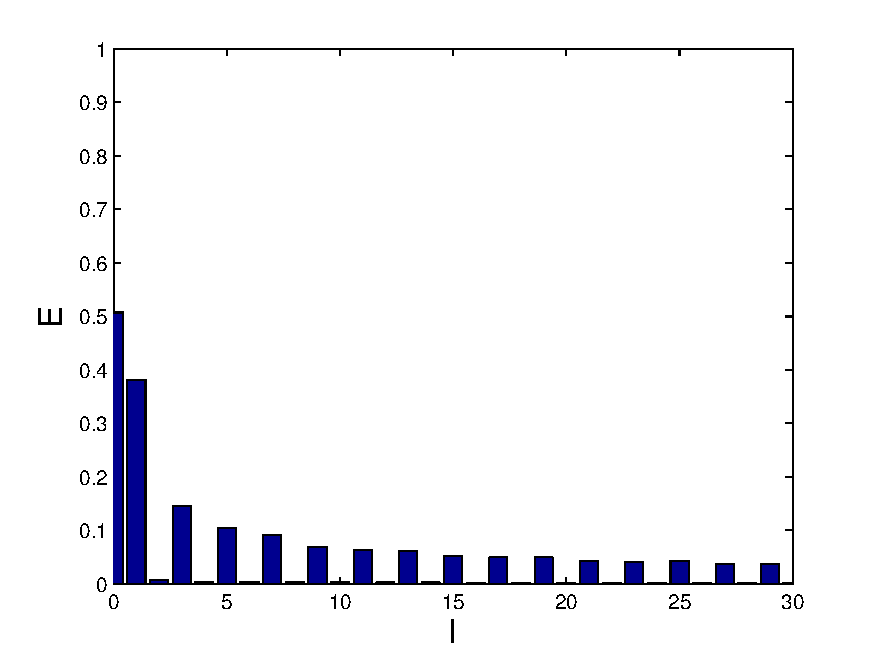
\includegraphics[width=0.45\textwidth]{kugel/kSpektrum/Kugel_1_2.pdf}
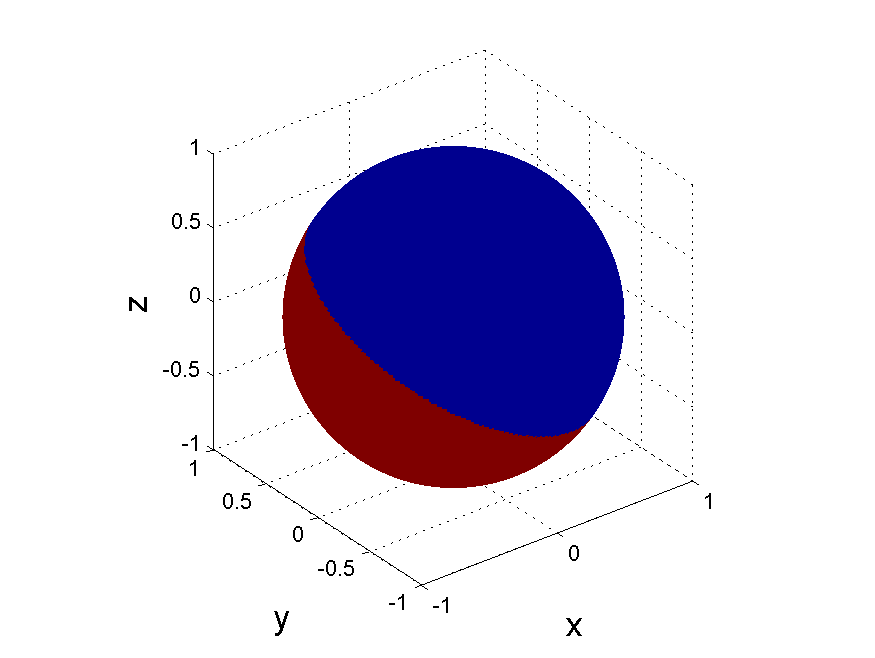
\includegraphics[width=0.45\textwidth]{kugel/kSpektrum/Kugel_2_1.pdf}
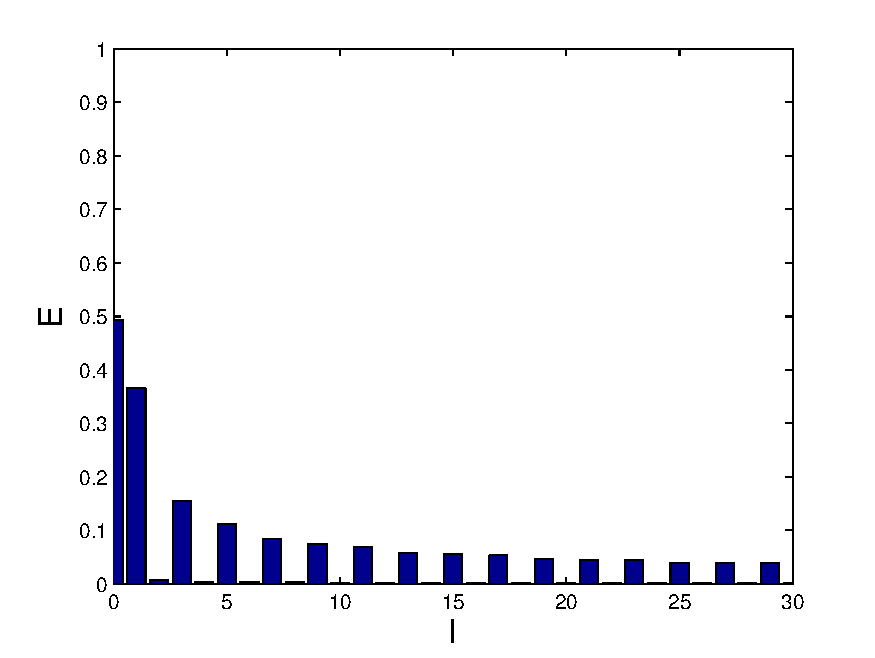
\includegraphics[width=0.45\textwidth]{kugel/kSpektrum/Kugel_2_2.pdf}
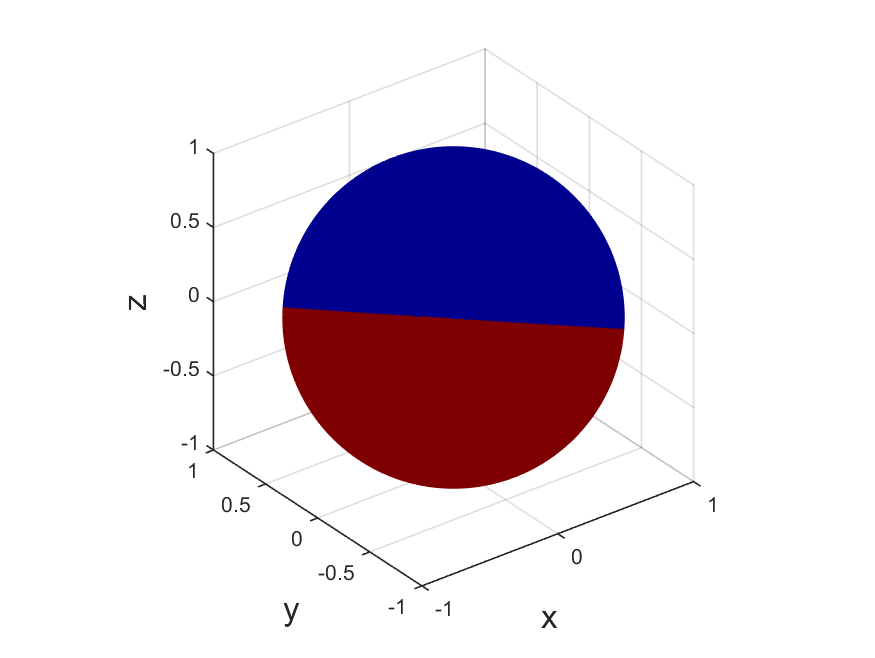
\includegraphics[width=0.45\textwidth]{kugel/kSpektrum/Kugel_3_1.pdf}
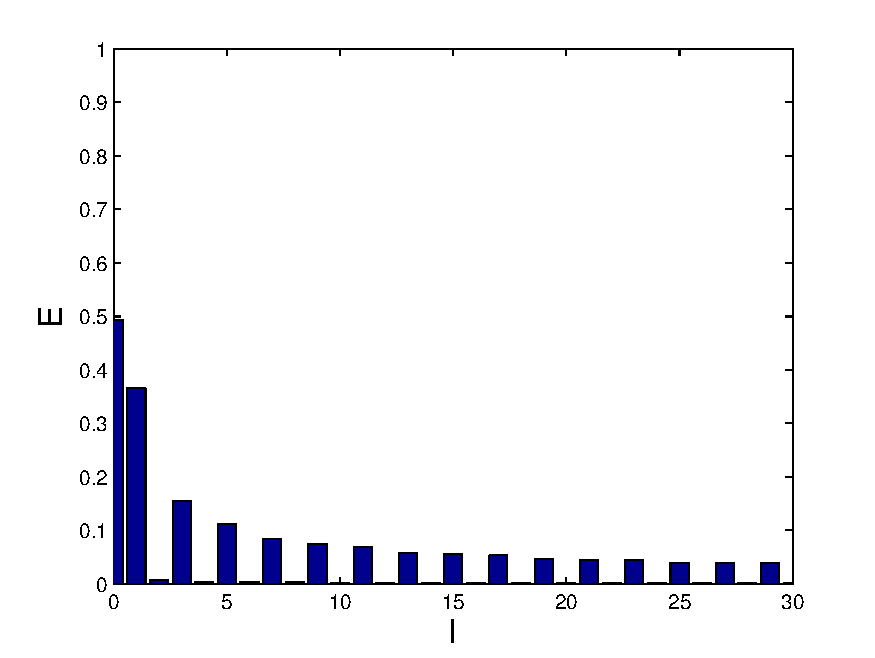
\includegraphics[width=0.45\textwidth]{kugel/kSpektrum/Kugel_3_2.pdf}
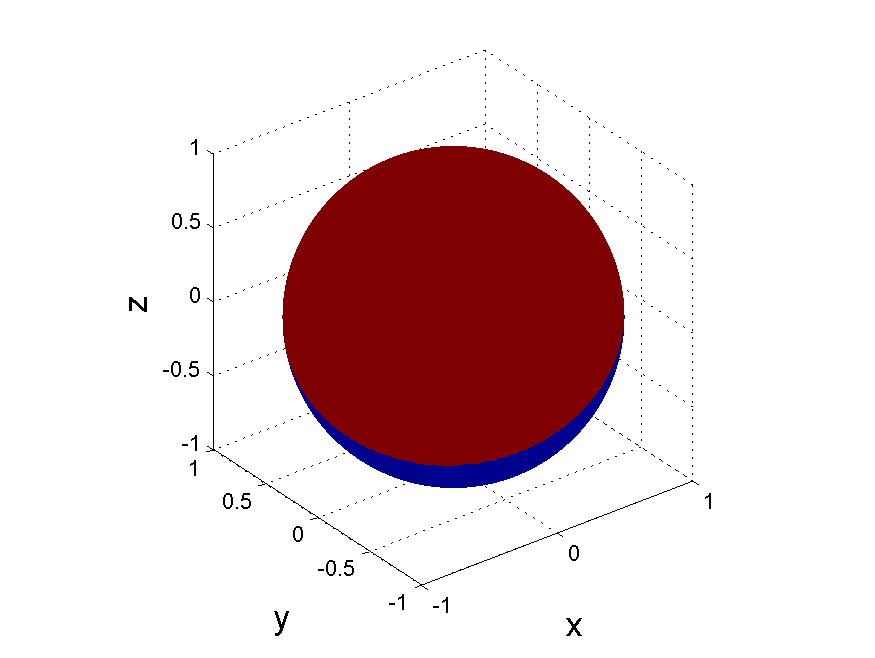
\includegraphics[width=0.45\textwidth]{kugel/kSpektrum/Kugel_4_1.pdf}
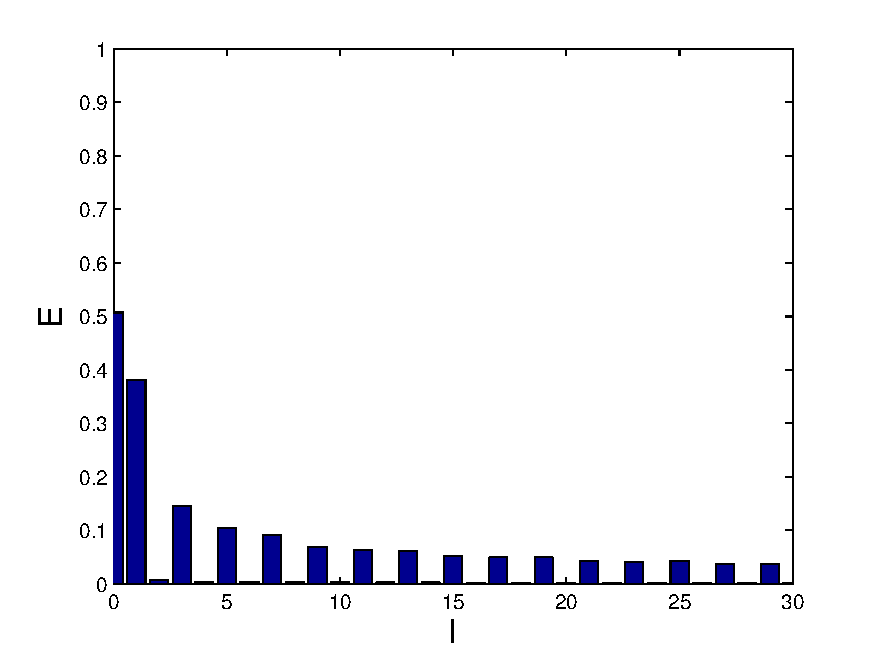
\includegraphics[width=0.45\textwidth]{kugel/kSpektrum/Kugel_4_2.pdf}
\caption{Rotierende Funktion auf der Kugeloberfl"ache
\label{skript:Spektrum2}}
\end{figure}
